\documentclass[11pt,a4paper]{article}
\usepackage[T1]{fontenc}
\usepackage[utf8]{inputenc}
\usepackage{lmodern,microtype}
\usepackage{amsmath,amssymb,amsthm,mathtools,bm}
\usepackage{booktabs,array,tabularx,longtable}
\usepackage{graphicx,float,caption,xcolor}
\usepackage[margin=2.15cm]{geometry}
\usepackage{enumitem,fancyhdr}
\usepackage[hidelinks,pdfencoding=auto]{hyperref}

\hypersetup{
 pdftitle={FIN ST263--ST277: Spontaneous Phase Orbits, Certified Selection, and Trace-Class Obstructions},
 pdfauthor={Krzysztof Żuchowski},
 pdfsubject={Analytical, exact, interval, and computational execution of FIN programs ST263--ST277},
 pdfkeywords={FIN, fractal information, D12 symmetry, spontaneous symmetry breaking, equivariant bifurcation, Krawczyk certificate, quantum recovery, refinement, log-Haar measure, trace class}
}

\definecolor{proved}{RGB}{20,92,48}
\definecolor{conditional}{RGB}{148,88,0}
\definecolor{blocked}{RGB}{150,28,28}
\newcommand{\Proven}{\textcolor{proved}{\textbf{[PROVEN]}}}
\newcommand{\Evidence}{\textcolor{conditional}{\textbf{[STRONG NUMERICAL EVIDENCE]}}}
\newcommand{\Conditional}{\textcolor{conditional}{\textbf{[CONDITIONAL]}}}
\newcommand{\Blocked}{\textcolor{blocked}{\textbf{[BLOCKED]}}}
\newcommand{\R}{\mathbb R}
\newcommand{\C}{\mathbb C}
\newcommand{\Tr}{\operatorname{tr}}
\newtheorem{theorem}{Theorem}[section]
\newtheorem{proposition}[theorem]{Proposition}

\pagestyle{fancy}\fancyhf{}
\lhead{FIN ST263--ST277}\rhead{Release 10.75}\cfoot{\thepage}
\setlength{\headheight}{14pt}
\setlist[itemize]{leftmargin=1.3em,itemsep=2pt,topsep=3pt}
\setlist[enumerate]{leftmargin=1.5em,itemsep=2pt,topsep=3pt}
\sloppy

\begin{document}
\hypersetup{pageanchor=false}
\begin{titlepage}
\centering
\vspace*{1cm}
{\Large Fractal Information Theory Project\par}
\vspace{.9cm}
{\huge\bfseries FIN ST263--ST277\par}
\vspace{.4cm}
{\LARGE Spontaneous Phase Orbits, Certified Selection,\par}
{\LARGE and Trace-Class Obstructions\par}
\vspace{1cm}
{\large Analytical, exact, interval, and computational research report\par}
\vfill
{\Large Krzysztof \.{Z}uchowski\par}
\vspace{.2cm}
{\large Independent Researcher --- Fractal Information Theory Project\par}
{\large ORCID: 0009-0002-0909-3613\par}
\vspace{.8cm}
{\large August 12, 2026\par}
\vspace{.3cm}
{\large Release 10.75\par}
\vfill
\begin{minipage}{.92\textwidth}\small
\textbf{Repository snapshot.} The audited tracked base is commit
\texttt{10d0ccc19ac7b9101c7d382dd0859b352cec802f}. The working tree contains
uncommitted and untracked research artifacts; reproducibility therefore depends on the
accompanying SHA-256 manifest as well as the tracked base.

\medskip
\textbf{License.} CC BY 4.0. \quad \textbf{Language.} English. \quad
\textbf{Resource type.} Preprint and executable reproducibility package.
\end{minipage}
\end{titlepage}
\hypersetup{pageanchor=true}\pagenumbering{roman}

\begin{abstract}
Programs ST263--ST277 attack three connected questions left by Release 10.74: whether a
symmetry-broken state can arise without contradicting the strict $D_{12}$ symmetry, whether
the selector and refinement calculations can be certified more strongly, and whether the
log-Haar scale plateau admits a mathematically controlled infinite completion.

The central constructive result is precise but conditional. The strict operator canonically
determines a two-dimensional lowest positive Fourier eigenspace, hence a phase circle. The
invariant algebra of $D_{12}$ has no anisotropic scalar below degree twelve; its first such
term is $\operatorname{Re}z^{12}$. Therefore a potential $-\kappa\operatorname{Re}z^{12}$
with $\kappa>0$ has exactly twelve stable angular branches. A single realization breaks
symmetry while their uniform ensemble restores it. However, neither $\kappa$, the nonzero
radius, nor the realized phase follows from the strict operator. This is a minimal admissible
mechanism for spontaneous selection, not a discharge of the selector obstruction.

Among the closure results, ST267 converts the previously numerical selector schedule into a
unique global solution of the declared ten-knot discretized convex problem by an outward
Krawczyk certificate for its active-set KKT system. ST268 proves the flat mean-zero affine
connection natural under every exact linear-isometric refinement. ST269 certifies the full
halfwidth-$0.00070$ nuisance cube and locates the fixed-resolution method boundary at the
next declared radius. ST271 gives an exact continuum counterexample showing that two
positive marginal Clifford gaps do not ensure joint uniqueness.

The strongest negative multiscale result is ST275: a nonzero exactly scale-invariant
log-Haar distribution over all positive rates cannot have a trace-class heat completion,
because its heat trace diverges logarithmically at zero. Cutoffs yield a controlled plateau
with an explicit error bound but necessarily break exact scale invariance. No physical
clock, length, Planck scale, spacetime, laboratory record, legacy-role transfer, Standard
Model, gravity, or Theory-of-Everything closure is claimed.
\end{abstract}

\tableofcontents\newpage\pagenumbering{arabic}

\section{Scope and proof discipline}

The strict working operator remains
\[
A=sI-W,\qquad W_{xx}=0,\qquad
W_{xy}=K_{\rm strict}(d(x,y))\quad(x\ne y),
\]
with $A\bm 1=0$ and $A\succeq0$. The diagonal exclusion is part of the definition. The
historical $K_{\rm legacy,ont}$ remains an intermediate bridge kernel. No legacy physical
role is transferred to the strict kernel in this report.

\begin{itemize}
\item \Proven{} means an exact deduction or a stated finite outward certificate.
\item \Conditional{} means a theorem whose additional carrier, coefficient, cutoff, bath,
or naturality premise is displayed explicitly.
\item \Evidence{} means a reproducible numerical result without a global certificate.
\item \Blocked{} means an evidentiary input is absent and is not replaced by simulation.
\end{itemize}

The nadsoliton is retained as the primordial fractal information in a solitonic state; no
lower information layer is introduced. This ontological statement is not used as a premise
in any mathematical proof below.

\section{Executive result ledger}

\small
\begin{longtable}{p{.075\textwidth}p{.27\textwidth}p{.55\textwidth}}
\toprule
Program & Status & Result \\
\midrule\endhead
ST263 & \Conditional & Strict lowest-mode circle; first anisotropic invariant
$\operatorname{Re}z^{12}$; twelve conditional stable phases. \\
ST264 & \Proven & Complete seven-generator polynomial equivariant module through degree 11. \\
ST265 & \Proven & Forty-four new interval boxes; no collision or stationary-rank loss on the targeted segment. \\
ST266 & \Proven & Rational global CPTP recovery optimum $3/8$ for a nonorthogonal measure-and-prepare channel. \\
ST267 & \Proven & Unique global optimum of the declared discrete selector-control problem. \\
ST268 & \Proven & Flat affine connection is unique and natural under exact linear-isometric refinements. \\
ST269 & \Proven & Complete $40^3$ cover at $0.00070$; fixed-resolution certificate fails at $0.00075$. \\
ST270 & \Proven & Distribution-free simultaneous finite-confidence rectangles under clustered counts. \\
ST271 & \Proven & Circle of global Clifford minimizers despite two positive marginal gaps. \\
ST272 & \Proven{} + \Evidence & Rigorous adaptive $s=1/2$ enclosure; Chernoff-$s$ optimizer remains numerical. \\
ST273 & \Conditional & Finite-controller reset cost $\beta W\ge h_2(p)$ when an uncertain record must be erased. \\
ST274 & \Conditional & Unlabelled-fiber naturality reduces refinement freedom from seven dimensions to one. \\
ST275 & \Proven & Finite-cutoff bound and impossibility of nonzero exact scale-invariant trace-class completion. \\
ST276 & \Proven & Frozen child-resolving instrument and record schema reconstruct the complement generator. \\
ST277 & \Blocked & No independently registered event record exists. \\
\bottomrule
\end{longtable}
\normalsize

\section{ST263--ST264: spontaneous phase orbits without a hidden selector}

The smallest positive strict eigenvalue is
\[
\lambda_1=0.7541211542070798
\]
with real multiplicity two. Thus $A$ canonically gives a carrier $E_1\cong\C$, but it acts
as $\lambda_1 I$ on that carrier and cannot choose a phase. Write the $D_{12}$ action as
\[
z\longmapsto e^{2\pi i/12}z,\qquad z\longmapsto\bar z.
\]

\begin{theorem}[minimal anisotropic invariant]
Every real scalar $D_{12}$-invariant polynomial of degree below twelve is radial on $E_1$.
The first anisotropic invariant is $\operatorname{Re}z^{12}$. Conditional on a fixed radius
$r>0$ and $\kappa>0$, the angular potential
\[
V_{\rm phase}(z)=-\kappa\operatorname{Re}z^{12}
\]
has exactly twelve stable angular minima.
\end{theorem}

The constructed probability branches are positive: their entries range from
$0.0343435$ to $0.1323231$. Every branch has a reflection stabilizer of order two, whereas
the equal ensemble of all twelve branches is uniform to $2\times10^{-17}$. This is the
mathematically correct sense in which a symmetric law may permit individually broken
realizations. It does not mean that symmetry itself is feedback: the radial instability and
the anisotropic coefficient must still be generated by a dynamical law.

\begin{figure}[H]\centering
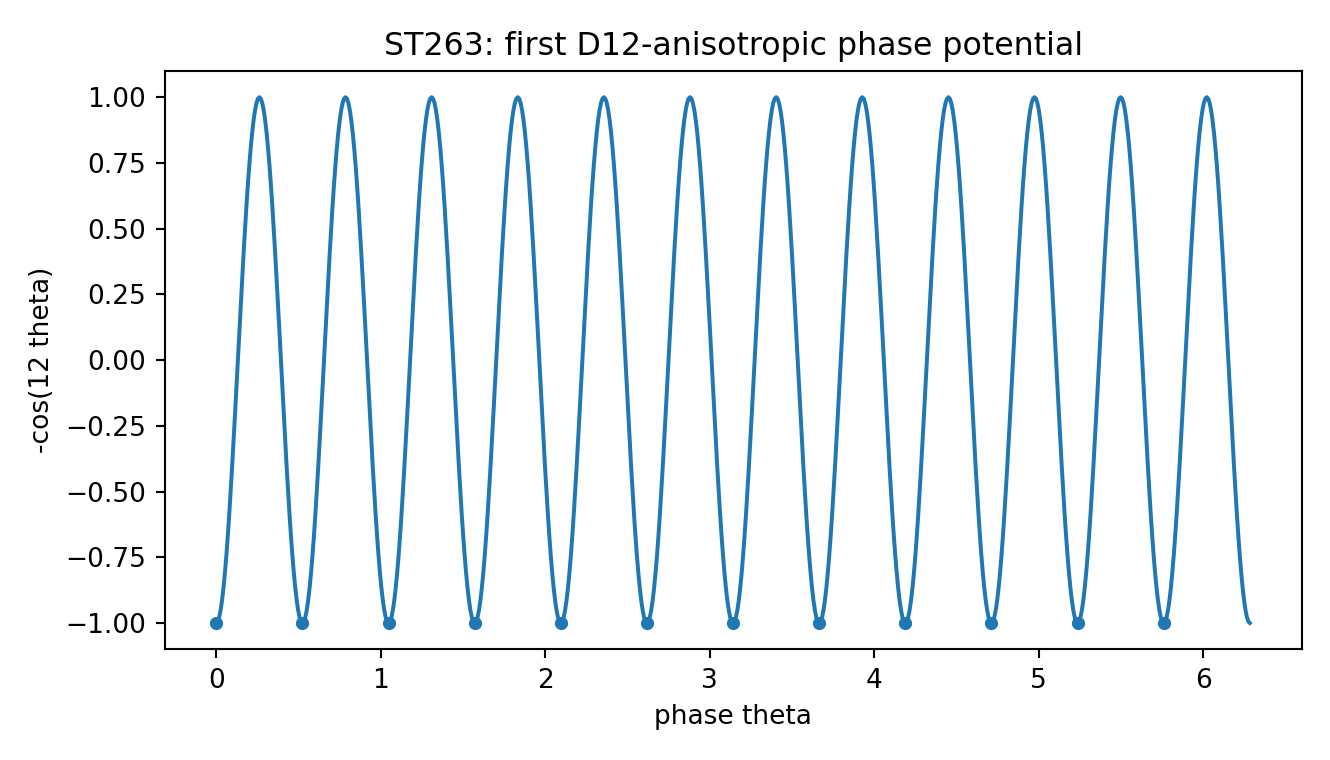
\includegraphics[width=.78\textwidth]{FIN_ST263_ST277_Figures/st263_phase_orbit.png}
\caption{The first symmetry-allowed anisotropic phase potential has twelve equivalent minima.}
\end{figure}

ST264 sharpens the response classification. Through degree eleven, the real
reflection-compatible $D_{12}$-equivariant module $F:E_1\to E_1$ has the seven monomials
\[
z,\ z|z|^2,\ z|z|^4,\ z|z|^6,\ z|z|^8,\ z|z|^{10},\ \bar z^{11}.
\]
The final generator is the first phase-sensitive one. Equivariance nevertheless implies
$\operatorname{Stab}(z)\subseteq\operatorname{Stab}(F(z))$: processing can amplify a
broken state, but cannot make its stabilizer smaller than that of its input. The missing
scientific atom is now explicit: a strict source for the nonlinear coefficient, nonzero
radius, and realized phase.

\section{ST265: targeted event exclusion}

The closest inherited nonfold seed pair, 20 and 23, was extended from step 8 to step 30.
All 44 new roots have outward pseudo-arclength Krawczyk certificates. Their minimum new
box clearance is $0.0183930$. The smallest interval lower bound on the full row rank of the
stationary Jacobian is
\[
2.05253993945\times10^{-5}>0.
\]
The rank margin approaches a small positive value and then reopens; on the certified finite
segment this is a near miss, not a collision or rank-loss event.

\begin{figure}[H]\centering
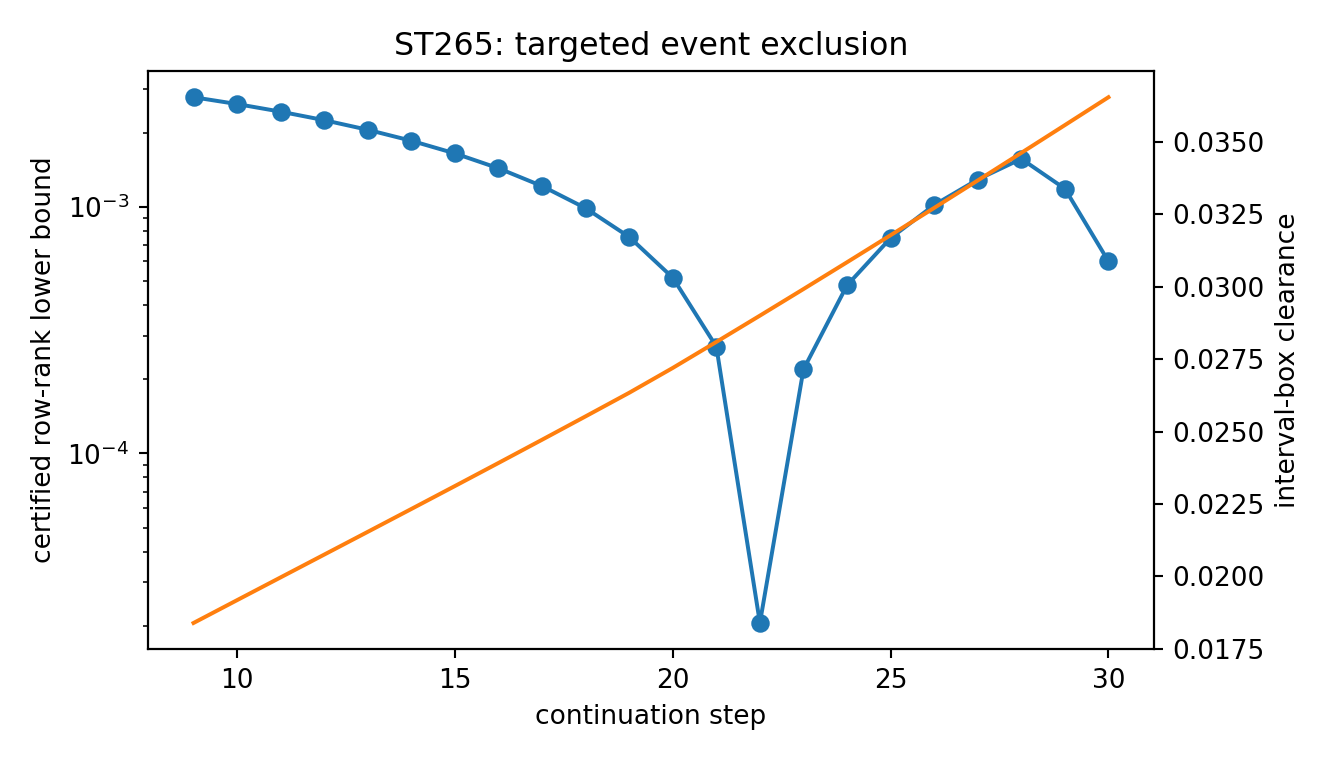
\includegraphics[width=.80\textwidth]{FIN_ST263_ST277_Figures/st265_event_audit.png}
\caption{Certified stationary-rank lower bound and separation of the targeted branch pair.}
\end{figure}

No conclusion is made about later continuation, distant components, stability, or particles.

\section{ST266: a recovery theorem outside the previous channel orbits}

Consider the channel that measures the computational basis and prepares
\[
\tau_0=\begin{pmatrix}1/2&3/10\\3/10&1/2\end{pmatrix},\qquad
\tau_1=\begin{pmatrix}9/10&0\\0&1/10\end{pmatrix}.
\]
The states are full rank and noncommuting. Optimizing recovery fidelity becomes binary state
discrimination. Since $\Delta=\tau_0-\tau_1$ has eigenvalues $\pm1/2$, the rational
Helstrom effect
\[
M_0=\begin{pmatrix}1/10&3/10\\3/10&9/10\end{pmatrix}
\]
attains discrimination sum $3/2$. The dual
$\Gamma=(\tau_0+\tau_1+|\Delta|)/2$ dominates both states and also has trace $3/2$.
Thus the global CPTP recovery optimum is
\[
F_e^{\rm opt}=\frac14\frac32=\frac38.
\]
The channel is nonunital, has Choi rank four, and has noncommuting outputs; these invariants
exclude unitary equivalence to a Pauli mixture or qubit amplitude damping.

\section{ST267: interval KKT closure of the selector model}

The ten-knot schedule from ST252 has exactly one active inequality: the final negative slew
face. Solving its 12-variable active KKT system gives
\[
J_*=0.4405461745248221,\qquad \mu_*=0.0577607478863>0.
\]
An outward Krawczyk box with knot radius $2\times10^{-9}$ and multiplier radius
$2\times10^{-8}$ has minimum inclusion margin
$1.99997\times10^{-9}$. The nearest inactive slew slack is $0.0358324$ and all box bounds
are inactive. The objective Hessian has minimum eigenvalue $0.492701$ at the root.

The entropy part is a sum of jointly convex Bernoulli Jeffreys divergences evaluated on
affine variables; endpoint KL terms and the quadratic slew term make the complete objective
strictly convex. Hence KKT sufficiency promotes the isolated root to the unique global
minimizer of the exact declared ten-knot, 600-step discretized model.

\begin{figure}[H]\centering
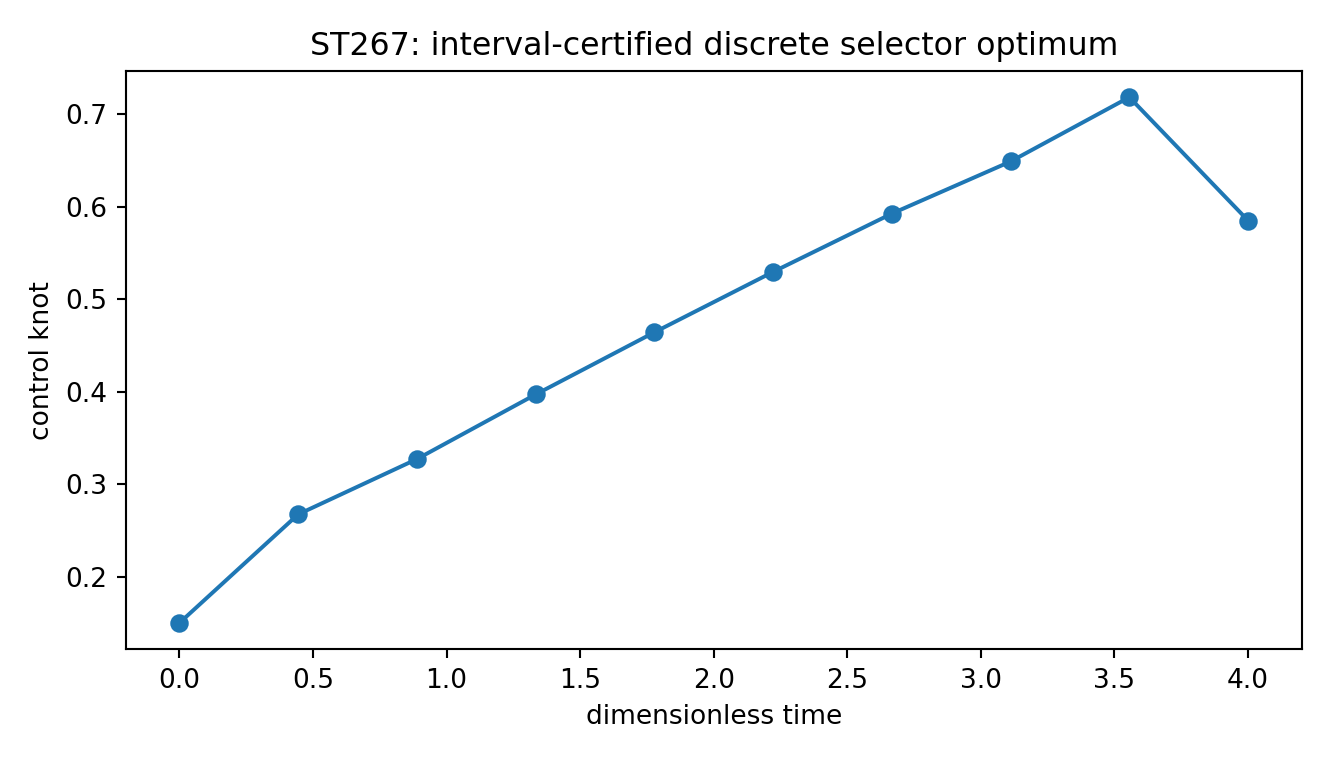
\includegraphics[width=.78\textwidth]{FIN_ST263_ST277_Figures/st267_selector_kkt.png}
\caption{The unique interval-certified optimum of the declared discrete selector model.}
\end{figure}

This does not source the preferred endpoint, bath, rate constant, dimensionless clock, or
physical energy unit.

\section{ST268--ST270: refinement naturality, certificate boundary, and confidence}

For an exact self-adjoint refinement
\[
\widetilde A=RAR^*\oplus B
\]
with normalized linear isometry $R$, one has
\[
g_{\widetilde A}(Ru,Rv)=g_A(u,v),\qquad
R(\nabla_uv)=\widetilde\nabla_{Ru}(Rv).
\]
Thus the flat mean-zero affine Levi--Civita connection is unique and natural under the
complete exact linear-isometric refinement class, including arbitrary positive complement
$B$. This remains a carrier theorem, not spacetime geometry.

ST269 evaluates a predeclared fixed-resolution continuation campaign. All
$40^3=64{,}000$ outward cells certify the nuisance cube of halfwidth $0.00070$; the minimum
margin is $2.12932459357\times10^{-4}$. At the next radius $0.00075$, five of eight corner
tiles fail. This refutes that proposed complete fixed-resolution cover but does not show
root loss.

\begin{figure}[H]\centering
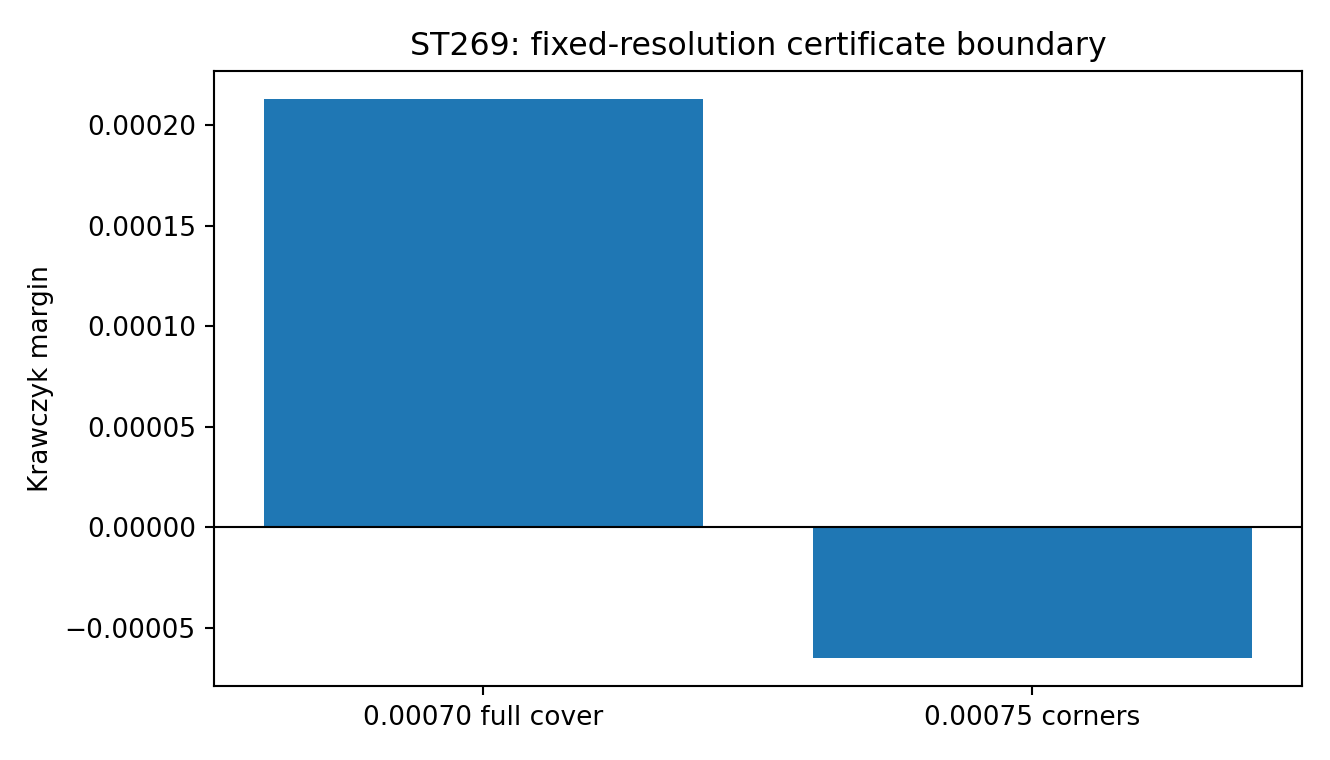
\includegraphics[width=.76\textwidth]{FIN_ST263_ST277_Figures/st269_nuisance_boundary.png}
\caption{Positive full-cover margin at $0.00070$ and the first failed fixed-resolution attempt.}
\end{figure}

ST270 treats every declared common-shock cluster as one independent bounded vector. A
two-sided Hoeffding bound and a union bound across six modes produce a simultaneous
$95\%$ confidence rectangle at every admissible parameter. This is distribution-free but
conservative; it relies on independent clusters, known attenuation, and the supplied count
model.

\section{ST271--ST272: falsifying a uniqueness heuristic and improving transfer bounds}

Let
\[
X_0=\frac35\sigma_z,\qquad Z_0=\frac45\sigma_z.
\]
Both targets have positive marginal sign gaps, but their Bloch columns are parallel. For
every unit $u_\phi$ perpendicular to $z$,
\[
X_\phi=\frac35\sigma_z+\frac45u_\phi,\qquad
Z_\phi=\frac45\sigma_z-\frac35u_\phi
\]
are anticommuting Hermitian involutions and attain the same global objective $2$. Therefore
the global minimizer set is a circle. Two marginal gaps alone are insufficient; the
full-column-rank hypothesis cannot be removed.

\begin{figure}[H]\centering
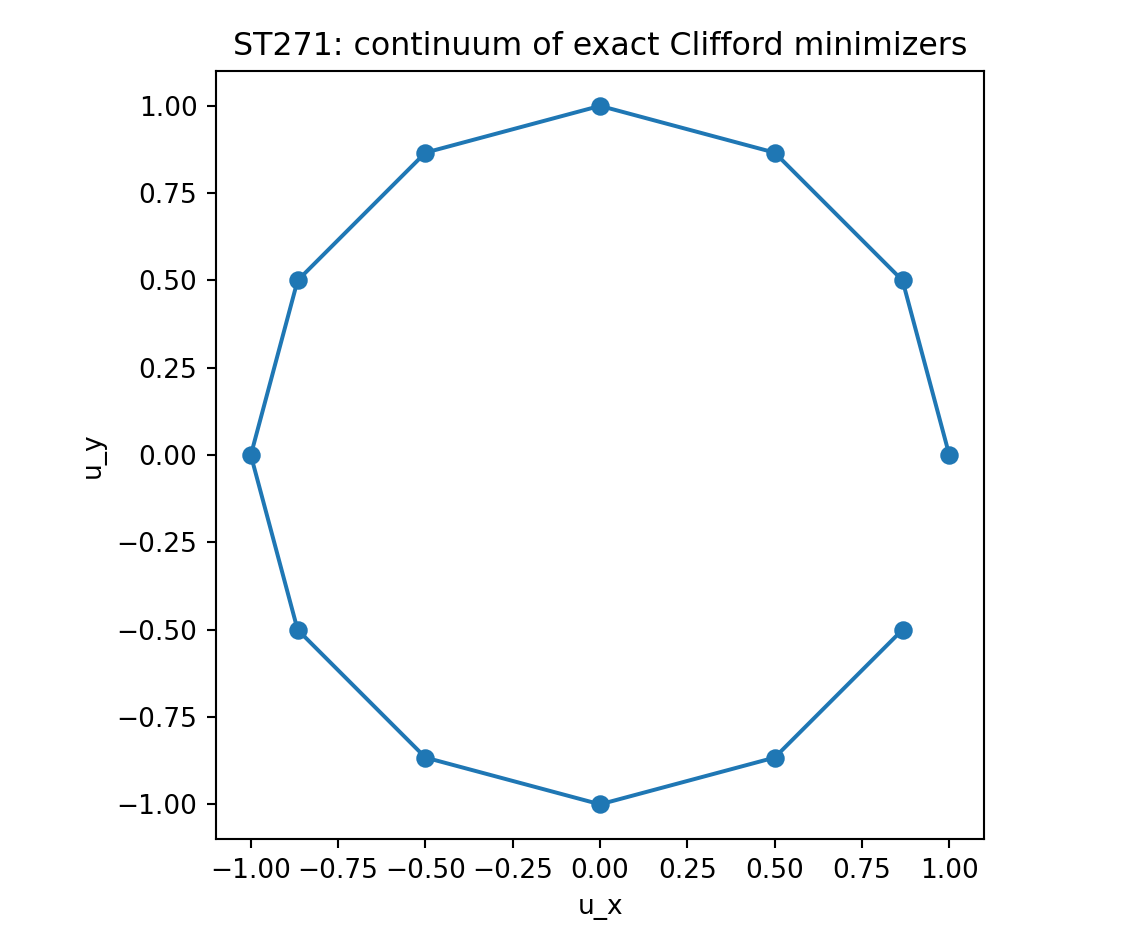
\includegraphics[width=.55\textwidth]{FIN_ST263_ST277_Figures/st271_clifford_circle.png}
\caption{An exact circle of globally minimizing Clifford pairs.}
\end{figure}

For the belief-transfer operator, three adaptive rounds reduce the spectral-radius interval
width from $0.0556162$ to $0.0509913$. The rigorous fixed-$s=1/2$ rate interval is
\[
[0.7129988031061385,\ 0.8228442593887783].
\]
Intersecting it with the independent earlier certificate gives
\[
[0.7129988031061385,\ 0.8198470892461787].
\]
Finite-depth point collocation suggests $s\approx0.5007394167$, but no all-$s$ interval
derivative certificate was produced; this candidate remains \Evidence.

\section{ST273--ST274: controller and refinement resources}

A two-state controller implements an exact controlled-SWAP. If its program bit is known
and uncomputed reversibly, no positive universal Landauer cost follows. If the controller
retains an uncertain classical record $\operatorname{diag}(1-p,p)$ and must be restored to
a pure standard state in a bath, then
\[
\beta W_{\rm reset}\ge h_2(p).
\]
At $p=1/2$ the bound is $\ln2$. The bath, record law, and Hamiltonian are supplied; FIN does
not derive them.

ST274 adds one explicit categorical premise: each two-point refinement fiber is unlabelled,
so independent local $S_2$ relabellings are natural automorphisms. They exchange aligned
and crossed horizontal weights and force
\[
p_d=q_d=\frac{W_d}{2},\qquad d=1,\ldots,6.
\]
The seven-dimensional ST259 cone collapses to the single ray $v\ge0$ of vertical rates.
Because $v$ is invariant under all relabellings, naturality still does not select it. This
is a one-modulus obstruction, not a unique fractal refinement.

\section{ST275: controlled plateaus and a trace-class impossibility theorem}

For density $\rho$ and cutoffs $0<\mu_{\min}<\mu_{\max}<\infty$, the log-Haar fiber
contribution is exactly
\[
d_{\rm fib}(t)=2\rho\left[
\log(1+e^{-2\mu_{\min}t})-\log(1+e^{-2\mu_{\max}t})
\right].
\]
Its deficit from the ideal plateau obeys
\[
0\le2\rho\ln2-d_{\rm fib}(t)
\le2\rho\mu_{\min}t+2\rho e^{-2\mu_{\max}t}.
\]

\begin{theorem}[trace-class obstruction]
A nonzero exactly scale-invariant log-Haar density on all positive rates does not define a
trace-class heat completion for any $t>0$.
\end{theorem}

Indeed, the heat trace contains
\[
\int_0^\infty e^{-2\mu t}\rho\,\frac{d\mu}{\mu},
\]
which diverges logarithmically at $\mu=0$. A trace-class completion must introduce an
infrared cutoff or a density vanishing at zero. Either modification breaks exact scale
invariance. Therefore a finite visible scale plateau is mathematically possible, but an
exact infinite self-similar tower and trace-class dynamics cannot coexist in this model.

\begin{figure}[H]\centering
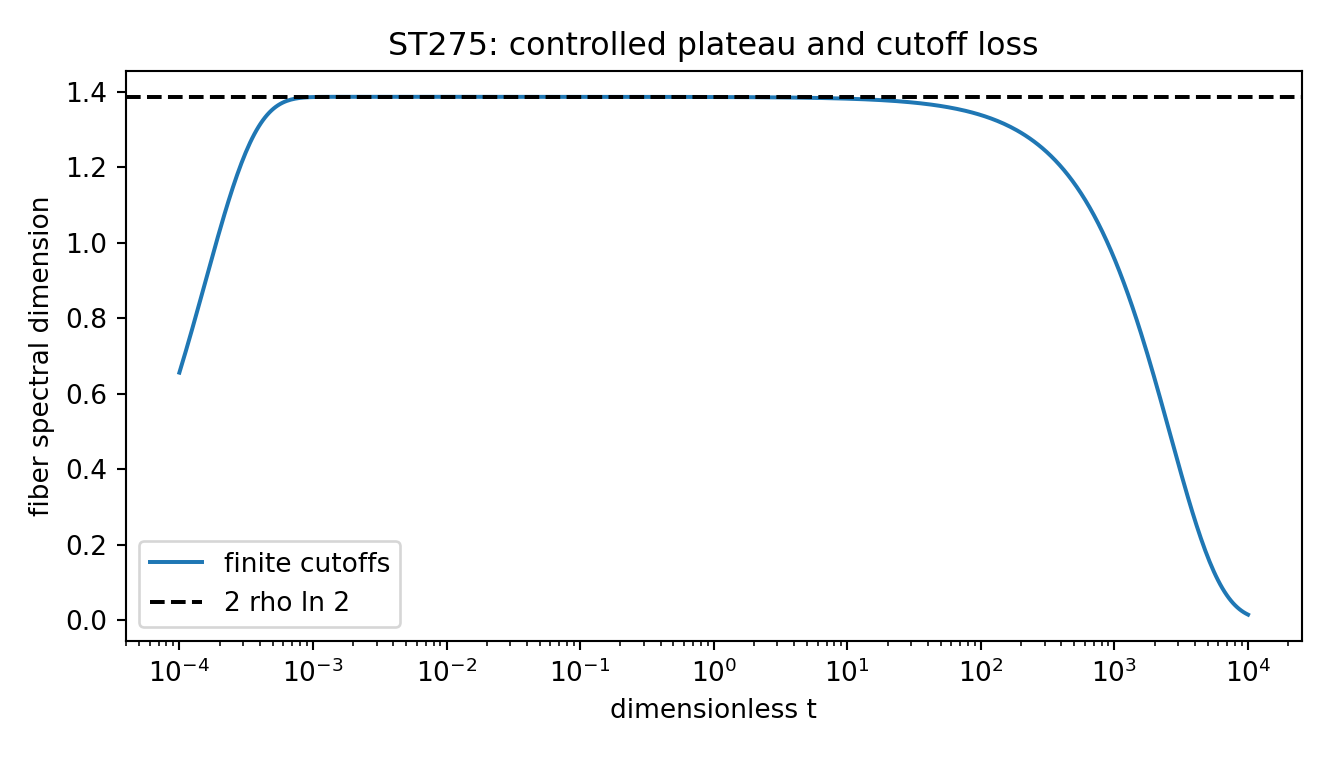
\includegraphics[width=.78\textwidth]{FIN_ST263_ST277_Figures/st275_cutoff_plateau.png}
\caption{A controlled finite-cutoff plateau; both ends expose the necessary scale breaking.}
\end{figure}

Nothing in this theorem identifies the cutoffs with physical length, Planck scale, octaves,
or legacy coupling formulas.

\section{ST276--ST277: executable observation boundary}

The frozen refinement instrument uses all 24 child-resolved preparations $(x,a)$ and all
24 child-resolved effects $(y,b)$. The positive count probabilities determine every entry
of $e^{-t\widetilde A}$. The signed contrast
\[
H_{\rm odd}(y,x)=\frac12\bigl(
P_{y0|x0}-P_{y0|x1}-P_{y1|x0}+P_{y1|x1}\bigr)
\]
equals $S^*e^{-t\widetilde A}S=e^{-tB}$. With calibrated $t$ and the stated principal-log
condition,
\[
B=-t^{-1}\log H_{\rm odd}.
\]
The numerical replay error is below $10^{-14}$.

The record schema freezes timestamps, preparation and effect labels, counts, run and
calibration hashes, provider, registrar, analyst, and holdout status. Provider, registrar,
and analyst must be distinct. ST277 remains \Blocked: no independently registered raw
event record exists, so no empirical claim is made.

\section{Falsification ledger and surviving interpretation}

\begin{longtable}{p{.27\textwidth}p{.31\textwidth}p{.34\textwidth}}
\toprule
Candidate claim & Falsification attempt & Surviving statement \\
\midrule\endhead
$A$ selects a phase & Functional calculus on the degenerate $E_1$ sector & $A$ selects the carrier, not a point on its phase circle. \\
Symmetry breaking must be inserted as a direction & Invariant-theory search & The minimal anisotropy has forced degree 12, but its coefficient and realized branch are unsourced. \\
Two spectral gaps imply joint Clifford uniqueness & Parallel full-gap targets & False: an exact circle of global minimizers exists. \\
Locality selects refinement & Independent fiber relabelling & Freedom shrinks to one positive vertical rate, not zero. \\
Exact log-Haar flow gives an infinite physical fractal & Heat-trace audit near $\mu=0$ & False without a cutoff or vanishing density; either breaks exact scale invariance. \\
Executable specification is evidence & Custody and record audit & False: ST277 remains blocked. \\
\bottomrule
\end{longtable}

The deepest statement surviving this batch is
\begin{align*}
A&\text{ canonically determines a symmetric carrier and its allowed response algebra},\\
A&\text{ does not determine the nonlinear source, realized branch, or physical scale}.
\end{align*}

This refines the information-first intuition. Representation-independent structure may be
encoded by the carrier, group action, operators, preparations, effects, and transformation
laws rather than by the spectrum alone. Different observational layers can hide complement
generators, but an explicitly richer instrument can recover them. Information is therefore
not shown to propagate ``without any carrier''; instead, the same operational structure may
be instantiated in different carriers once a representation functor and preserved
observables are supplied.

\section{Recommended programs ST278--ST292}

\begin{enumerate}
\item[\textbf{ST278}.] Derive the coefficient and radius of the
$\operatorname{Re}z^{12}$ potential from one strict nonlinear interaction, or prove a source
obstruction.
\item[\textbf{ST279}.] Compute a Hilbert basis for the complete nonlinear
$D_{12}$-equivariant module beyond degree eleven.
\item[\textbf{ST280}.] Continue seed 23 only through a certified minimum-rank event bracket,
with an explicit finite stop.
\item[\textbf{ST281}.] Generalize the exact measure-and-prepare recovery theorem to arbitrary
rational binary qubit outputs.
\item[\textbf{ST282}.] Independently replay ST267 with rational or arbitrary-precision
interval arithmetic.
\item[\textbf{ST283}.] Test affine-connection naturality under nonlinear refinement
embeddings or construct a counterexample.
\item[\textbf{ST284}.] Adaptively subdivide failed $0.00075$ nuisance cells to separate
resolution loss from a root boundary.
\item[\textbf{ST285}.] Replace Hoeffding rectangles with exact-mixture or empirical-Bernstein
clustered confidence sets.
\item[\textbf{ST286}.] Classify higher-dimensional joint Clifford nonuniqueness beyond the
qubit rank-one counterexample.
\item[\textbf{ST287}.] Certify the global Chernoff-$s$ optimizer with interval derivatives
and complete $s$ coverage.
\item[\textbf{ST288}.] Construct an autonomous finite controller and distinguish catalytic
from resetting costs.
\item[\textbf{ST289}.] Impose coassociativity on $12\to24\to48$ unlabelled-fiber refinements
and classify surviving vertical-rate moduli.
\item[\textbf{ST290}.] Classify near-Haar trace-class densities and prove the optimal
plateau-width versus trace-class tradeoff.
\item[\textbf{ST291}.] Build an executable validator for the frozen ST276 instrument and
custody schema.
\item[\textbf{ST292}.] Resume empirical validation only after independently registered raw
events exist.
\end{enumerate}

ST278 is the decisive theoretical continuation. If the degree-twelve coefficient and a
nonzero radius can be derived from a strict interaction without already importing a broken
state, FIN will have an internal symmetry-breaking dynamics, although it will still not
choose one realized branch deterministically. ST290 is the decisive multiscale continuation:
it should quantify how long an approximately scale-invariant visible plateau can coexist
with trace-class completion.

\section{Reproducibility and conclusion}

The executable source \texttt{fin\_st263\_st277\_research.py} writes the aggregate JSON,
CSV ledger, fifteen per-program packets, and eight figures. The independent live replay
\texttt{test\_fin\_st263\_st277.py} checks packet hashes, the invariant module, all 44
continuation inclusions, rational recovery duality, the live KKT residual and convexity,
the $64{,}000$-box cover count, confidence construction, Clifford counterexample, adaptive
transfer narrowing, refinement intertwining, trace bound, and operational reconstruction.

The batch produces a substantive but bounded advance. FIN now has an exact minimal
mathematical template for twelve-branch spontaneous selection and a proof that symmetry can
be restored at the ensemble level. It does not yet have the strict nonlinear law that makes
this template inevitable. It also has a controlled interpretation of visible fractal scale
plateaus, together with a proof that an exact infinite log-Haar tower is incompatible with
trace-class heat dynamics. Consequently, neither spontaneous selection nor fractal layering
may be promoted from a conditional mathematical mechanism to observed physics without the
missing source and operational bridges.

\end{document}
